\documentclass[ignorenonframetext,]{beamer}
\setbeamertemplate{caption}[numbered]
\setbeamertemplate{caption label separator}{: }
\setbeamercolor{caption name}{fg=normal text.fg}
\beamertemplatenavigationsymbolsempty
\usepackage{lmodern}
\usepackage{amssymb,amsmath}
\usepackage{ifxetex,ifluatex}
\usepackage{fixltx2e} % provides \textsubscript
\ifnum 0\ifxetex 1\fi\ifluatex 1\fi=0 % if pdftex
\usepackage[T1]{fontenc}
\usepackage[utf8]{inputenc}
\else % if luatex or xelatex
\ifxetex
\usepackage{mathspec}
\else
\usepackage{fontspec}
\fi
\defaultfontfeatures{Ligatures=TeX,Scale=MatchLowercase}
\fi
\usecolortheme{beaver}
% use upquote if available, for straight quotes in verbatim environments
\IfFileExists{upquote.sty}{\usepackage{upquote}}{}
% use microtype if available
\IfFileExists{microtype.sty}{%
\usepackage{microtype}
\UseMicrotypeSet[protrusion]{basicmath} % disable protrusion for tt fonts
}{}
\newif\ifbibliography
\usepackage{color}
\usepackage{fancyvrb}
\newcommand{\VerbBar}{|}
\newcommand{\VERB}{\Verb[commandchars=\\\{\}]}
\DefineVerbatimEnvironment{Highlighting}{Verbatim}{commandchars=\\\{\}}
% Add ',fontsize=\small' for more characters per line
\usepackage{framed}
\definecolor{shadecolor}{RGB}{248,248,248}
\newenvironment{Shaded}{\begin{snugshade}}{\end{snugshade}}
\newcommand{\KeywordTok}[1]{\textcolor[rgb]{0.13,0.29,0.53}{\textbf{{#1}}}}
\newcommand{\DataTypeTok}[1]{\textcolor[rgb]{0.13,0.29,0.53}{{#1}}}
\newcommand{\DecValTok}[1]{\textcolor[rgb]{0.00,0.00,0.81}{{#1}}}
\newcommand{\BaseNTok}[1]{\textcolor[rgb]{0.00,0.00,0.81}{{#1}}}
\newcommand{\FloatTok}[1]{\textcolor[rgb]{0.00,0.00,0.81}{{#1}}}
\newcommand{\ConstantTok}[1]{\textcolor[rgb]{0.00,0.00,0.00}{{#1}}}
\newcommand{\CharTok}[1]{\textcolor[rgb]{0.31,0.60,0.02}{{#1}}}
\newcommand{\SpecialCharTok}[1]{\textcolor[rgb]{0.00,0.00,0.00}{{#1}}}
\newcommand{\StringTok}[1]{\textcolor[rgb]{0.31,0.60,0.02}{{#1}}}
\newcommand{\VerbatimStringTok}[1]{\textcolor[rgb]{0.31,0.60,0.02}{{#1}}}
\newcommand{\SpecialStringTok}[1]{\textcolor[rgb]{0.31,0.60,0.02}{{#1}}}
\newcommand{\ImportTok}[1]{{#1}}
\newcommand{\CommentTok}[1]{\textcolor[rgb]{0.56,0.35,0.01}{\textit{{#1}}}}
\newcommand{\DocumentationTok}[1]{\textcolor[rgb]{0.56,0.35,0.01}{\textbf{\textit{{#1}}}}}
\newcommand{\AnnotationTok}[1]{\textcolor[rgb]{0.56,0.35,0.01}{\textbf{\textit{{#1}}}}}
\newcommand{\CommentVarTok}[1]{\textcolor[rgb]{0.56,0.35,0.01}{\textbf{\textit{{#1}}}}}
\newcommand{\OtherTok}[1]{\textcolor[rgb]{0.56,0.35,0.01}{{#1}}}
\newcommand{\FunctionTok}[1]{\textcolor[rgb]{0.00,0.00,0.00}{{#1}}}
\newcommand{\VariableTok}[1]{\textcolor[rgb]{0.00,0.00,0.00}{{#1}}}
\newcommand{\ControlFlowTok}[1]{\textcolor[rgb]{0.13,0.29,0.53}{\textbf{{#1}}}}
\newcommand{\OperatorTok}[1]{\textcolor[rgb]{0.81,0.36,0.00}{\textbf{{#1}}}}
\newcommand{\BuiltInTok}[1]{{#1}}
\newcommand{\ExtensionTok}[1]{{#1}}
\newcommand{\PreprocessorTok}[1]{\textcolor[rgb]{0.56,0.35,0.01}{\textit{{#1}}}}
\newcommand{\AttributeTok}[1]{\textcolor[rgb]{0.77,0.63,0.00}{{#1}}}
\newcommand{\RegionMarkerTok}[1]{{#1}}
\newcommand{\InformationTok}[1]{\textcolor[rgb]{0.56,0.35,0.01}{\textbf{\textit{{#1}}}}}
\newcommand{\WarningTok}[1]{\textcolor[rgb]{0.56,0.35,0.01}{\textbf{\textit{{#1}}}}}
\newcommand{\AlertTok}[1]{\textcolor[rgb]{0.94,0.16,0.16}{{#1}}}
\newcommand{\ErrorTok}[1]{\textcolor[rgb]{0.64,0.00,0.00}{\textbf{{#1}}}}
\newcommand{\NormalTok}[1]{{#1}}
\usepackage{longtable,booktabs}
\usepackage{caption}
% These lines are needed to make table captions work with longtable:
\makeatletter
\def\fnum@table{\tablename~\thetable}
\makeatother
\usepackage{graphicx,grffile}
\makeatletter
\def\maxwidth{\ifdim\Gin@nat@width>\linewidth\linewidth\else\Gin@nat@width\fi}
\def\maxheight{\ifdim\Gin@nat@height>\textheight0.8\textheight\else\Gin@nat@height\fi}
\makeatother
% Scale images if necessary, so that they will not overflow the page
% margins by default, and it is still possible to overwrite the defaults
% using explicit options in \includegraphics[width, height, ...]{}
\setkeys{Gin}{width=\maxwidth,height=\maxheight,keepaspectratio}

% Prevent slide breaks in the middle of a paragraph:
\widowpenalties 1 10000
\raggedbottom

\AtBeginPart{
\let\insertpartnumber\relax
\let\partname\relax
\frame{\partpage}
}
\AtBeginSection{
\ifbibliography
\else
\let\insertsectionnumber\relax
\let\sectionname\relax
\frame{\sectionpage}
\fi
}
\AtBeginSubsection{
\let\insertsubsectionnumber\relax
\let\subsectionname\relax
\frame{\subsectionpage}
}

\setlength{\parindent}{0pt}
\setlength{\parskip}{6pt plus 2pt minus 1pt}
\setlength{\emergencystretch}{3em}  % prevent overfull lines
\providecommand{\tightlist}{%
\setlength{\itemsep}{0pt}\setlength{\parskip}{0pt}}
\setcounter{secnumdepth}{0}
%%% Работа с русским языком
\usepackage[russian,english]{babel}   %% загружает пакет многоязыковой вёрстки
\usepackage{fontspec}      %% подготавливает загрузку шрифтов Open Type, True Type и др.
\defaultfontfeatures{Ligatures={TeX},Renderer=Basic,Scale=0.75}  %% свойства шрифтов по умолчанию
\setmainfont[Ligatures={TeX,Historic}]{Times New Roman} %% задаёт основной шрифт документа
\setsansfont[Ligatures={TeX,Historic}]{Verdana} %% задаёт шрифт без засечек
\setmonofont[Scale=0.7]{DejaVu Sans Mono}

\linespread{0.75}

\definecolor{links}{HTML}{2A1B81}
\hypersetup{colorlinks=true,linkcolor=,urlcolor=links,pdfview=FitH,pdfpagelayout=SinglePage, unicode=true,breaklinks=true}

% links format
\usepackage{hyperref}

% decrease text margins
\setbeamersize{text margin left = 8pt, text margin right = 16pt}

\newcommand{\columnsbegin}{\begin{columns}}
\newcommand{\columnsend}{\end{columns}}
\newcommand{\blockbegin}{\begin{block}}
\newcommand{\blockend}{\end{block}}

\usepackage{graphics}

% % subfigures
% \usepackage{subcaption}
% \usepackage{wrapfig}

%\addto{\captionsrussian}{\renewcommand*{\figurename}{рис.}}

% Tables
% Define new column types to adjust sizes in tabular environment
% For example, \begin{tabular}{ L{2.3cm} C{2cm} C{1.5cm} C{2.5cm} C{4cm}}
\usepackage{array}
\renewcommand{\arraystretch}{2}
\newcolumntype{L}[1]{>{\raggedright\let\newline\\\arraybackslash\hspace{0pt}}m{#1}}
\newcolumntype{C}[1]{>{\centering\let\newline\\\arraybackslash\hspace{0pt}}m{#1}}
\newcolumntype{R}[1]{>{\raggedleft\let\newline\\\arraybackslash\hspace{0pt}}m{#1}}

\logo{
\includegraphics[height=0.3cm]{assets/Linmod_logo.png}}

\title{Линейные модели для счетных данных}
\subtitle{Линейные модели\ldots{}}
\author{Вадим Хайтов, Марина Варфоломеева}
\date{}

\begin{document}
\frame{\titlepage}

\begin{frame}{Мы рассмотрим}

\begin{itemize}
\tightlist
\item
  Различные варианты анализа, применяющегося для тех случаев, когда
  зависимая перменная - счетная величина (целые неотрицательные числа)
\end{itemize}

\begin{block}{Вы сможете}

\begin{itemize}
\tightlist
\item
  Объяснить особенности разных типов распределений, принадлежащих
  экспоненциальному семейству.
\item
  Построить пуасоновскую и квази-пуассоновскую линейную модель
\item
  Объяснить проблемы, связанные с избыточностью дисперсии в модели
\item
  Построить модель, основанную на отрицательном биномиальном
  распределении
\end{itemize}

\end{block}

\end{frame}

\section{Различные типы распределений}\label{--}

\begin{frame}{Распределение}

То, что мы в быту привыкли называть \textbf{распределением} - это
функция плотности вероятности.

\textbf{Плотность вероятности} - это функция, описывающая вероятность
получения разных значений случайной величины

\end{frame}

\begin{frame}{Нормальное распределение}

\columnsbegin

\column{0.5\textwidth}

\[f(y;\mu, \sigma)= \frac {1}{\sigma \sqrt{2 \pi}} e^{-\frac{(y-\mu)^2}{2\sigma^2}}\]

\textbf{Два параметра} (\(\mu\), \(\sigma\))

\it {Среднее}:  $E(Y)  = \mu$

\it {Дисперсия}: $var(Y) = \sigma^2$

\textbf {Пределы варьирования}

\(-\infty \le Y \le +\infty\)

\column{0.5\textwidth}

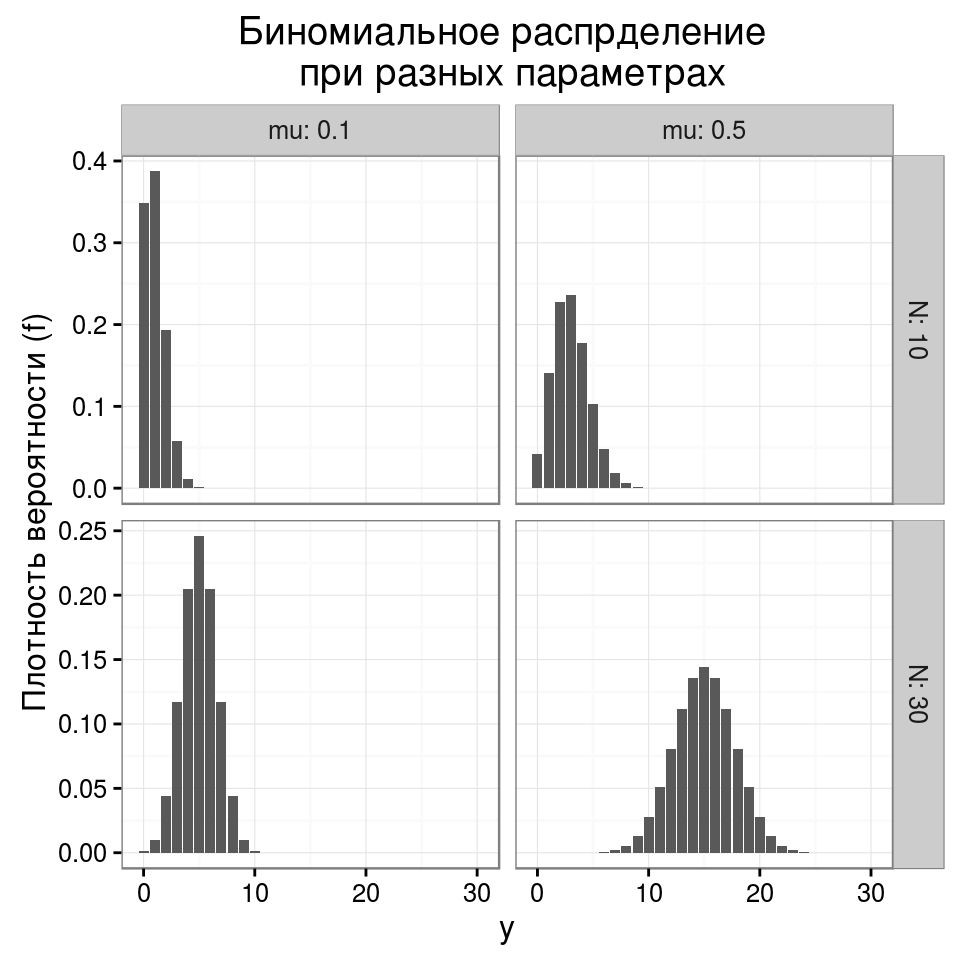
\includegraphics{12_GLM_count2_files/figure-beamer/unnamed-chunk-1-1.pdf}

\columnsend

\end{frame}

\begin{frame}{Распределение Пуассона}

\columnsbegin

\column{0.5\textwidth}

\[f(y;\mu)= \frac{\mu^y \times e{-\mu}}{y!}\]

\textbf {Один параметр} (\(\mu\))

\it Среднее: $E(Y)  = \mu$

\it Дисперсия: $var(Y) = \mu$

\textbf {Важное свойство}: При увеличении значения \(\mu\) увеличивается
размах варьирования

\textbf{Пределы варьирования}

\(0 \le Y \le +\infty\),\\
\(Y\) целочисленные!

\column {0.t \textwidth}
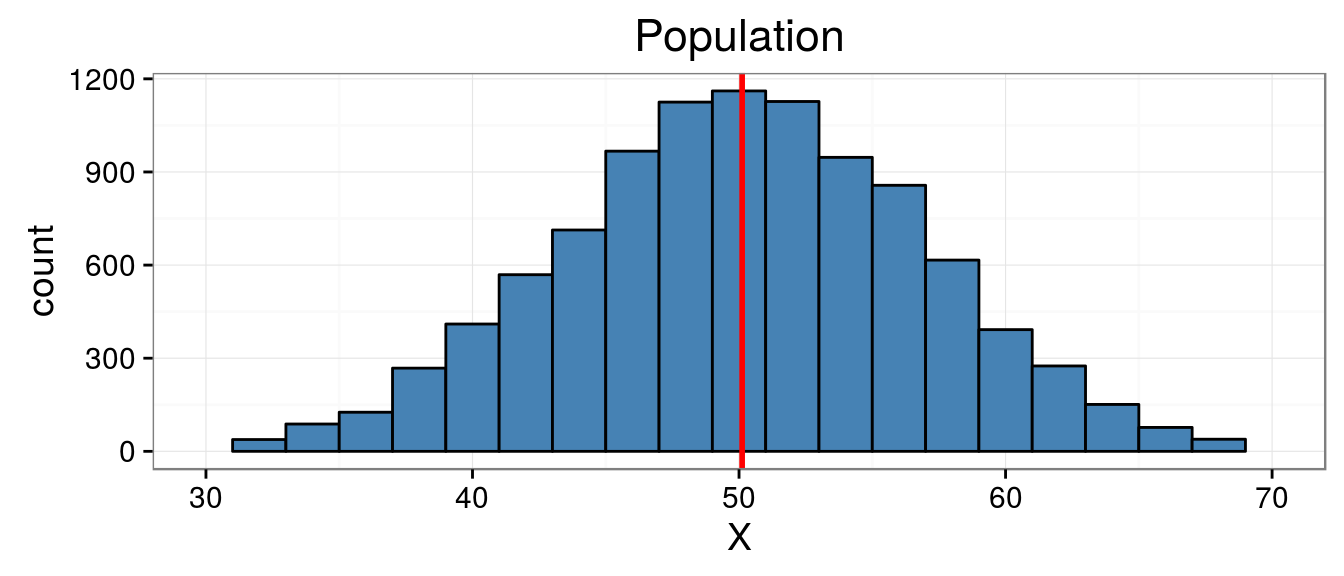
\includegraphics{12_GLM_count2_files/figure-beamer/unnamed-chunk-2-1.pdf}

\coumnsend

\end{frame}

\begin{frame}{Слайд с некрасивой таблицей в rmarkdown}

\begin{longtable}[]{@{}lll@{}}
\toprule
\begin{minipage}[b]{0.09\columnwidth}\raggedright\strut
Строки\strut
\end{minipage} & \begin{minipage}[b]{0.08\columnwidth}\raggedright\strut
Столбец 1\strut
\end{minipage} & \begin{minipage}[b]{0.08\columnwidth}\raggedright\strut
Столбец 2 с длинным предлинным названием\strut
\end{minipage}\tabularnewline
\midrule
\endhead
\begin{minipage}[t]{0.09\columnwidth}\raggedright\strut
Строка 1\strut
\end{minipage} & \begin{minipage}[t]{0.08\columnwidth}\raggedright\strut
Ячейка 1\strut
\end{minipage} & \begin{minipage}[t]{0.08\columnwidth}\raggedright\strut
Ячейка 2\strut
\end{minipage}\tabularnewline
\begin{minipage}[t]{0.09\columnwidth}\raggedright\strut
Строка 2 с длинным названием\strut
\end{minipage} & \begin{minipage}[t]{0.08\columnwidth}\raggedright\strut
Ячейка с длинным содержимым\strut
\end{minipage} & \begin{minipage}[t]{0.08\columnwidth}\raggedright\strut
Ячейка с еще более длинным содержимым\strut
\end{minipage}\tabularnewline
\bottomrule
\end{longtable}

\end{frame}

\begin{frame}{Слайд с красивой таблицей в LATEX}

\resizebox{1\textwidth}{!}{
\begin{tabular}{L{0.25\textwidth} C{0.25\textwidth} C{0.25\textwidth} C{0.25\textwidth}}
\hline\noalign{\smallskip}
Строки & Столбец 1 & Столбец 2 с длинным предлинным названием \\
\hline\noalign{\smallskip}
Строка 1 & Ячейка 1 & Ячейка 2 \\
Строка 2 с длинным названием & Ячейка с длинным содержимым & Ячейка с еще более длинным содержимым \\
\hline\noalign{\smallskip}
\end{tabular}
}

\end{frame}

\begin{frame}[fragile]{Двухколоночный слайд с рисунком и подписью мелким
шрифтом внизу}

Фрагментация лесных местообитаний - одна из важнейших проблем Австралии.
Вопрос: от каких факторов зависит обилие птиц во фрагментированных
лесных массивах? (Loyn, 1987)

\columnsbegin

\column{0.5\textwidth}

\textbf{Зависимая перменная}

\begin{itemize}
\tightlist
\item
  \texttt{ABUND} - Обилие птиц на стандартном маршруте
\end{itemize}

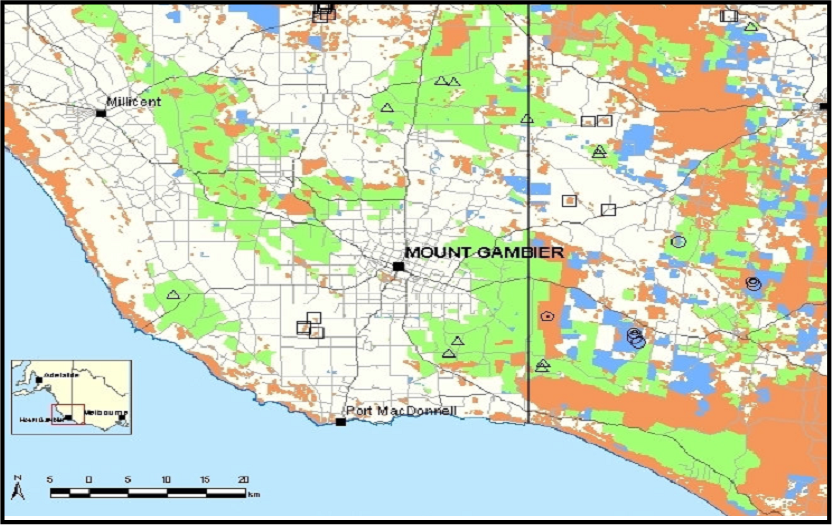
\includegraphics[width=\linewidth]{images/Australia.png}

\column{0.5\textwidth}

\textbf{Предикторы}

\begin{itemize}
\tightlist
\item
  \texttt{AREA} - площадь лесного массива (Га)\\
\item
  \texttt{YRISOL} - год, в котором произошла изоляция лесного массива\\
\item
  \texttt{DIST} - расстояние до ближайшего лесного массива (км)\\
\item
  \texttt{LDIST} - расстояние до ближайшего более крупного массива
  (км)\\
\item
  \texttt{GRAZE} - качественная оценка уровня выпаса скота (1 - низкий
  уровень, 5 - высокий уровень)\\
\item
  \texttt{ALT} - высота над уровнем моря (м)
\end{itemize}

\columnsend

\vskip0pt plus 1filll
\tiny{Пример из кн. Quinn, Keugh, 2002, данные из Loyn, 1987)}

\end{frame}

\begin{frame}[fragile]{Слайд с графиком с подписями}

\begin{Shaded}
\begin{Highlighting}[]
\KeywordTok{plot}\NormalTok{(pressure, }
     \DataTypeTok{xlab =} \StringTok{"Температура"}\NormalTok{, }
     \DataTypeTok{ylab =} \StringTok{"Давление"}\NormalTok{, }
     \DataTypeTok{main =} \StringTok{"Название графика кирилицей"}\NormalTok{)}
\end{Highlighting}
\end{Shaded}

\includegraphics[height=4cm]{12_GLM_count2_files/figure-beamer/pressure-1}

\end{frame}

\end{document}
